\documentclass[12pt]{beamer}

\usepackage[latin1]{inputenc}
\usepackage{amsmath}
\usepackage{amsfonts}
\usepackage{amssymb}
\usepackage{wrapfig}


\title[]{Realtime GPU-Accelerated Smoothed Particle Hydrodynamics with Bidirectional Rigid Body Coupling}
%\subtitle{Fluid Simulation for Games and Movies}
\author{Shaun Silson}

\date{27 April 2013}
\institute[UCT]{University of Cape Town}

\usetheme{Berkeley}
%\usetheme{Rochester}
%\usetheme{Darmstadt}

\usecolortheme{albatross}
\usecolortheme{orchid}



\begin{document}

\titlepage

\begin{frame}{Wait... WHAT!}


\begin{center}


\includegraphics[scale=0.5]{confused-girl} \pause

Watch This 

\end{center}

\end{frame}

%------------------------------------------------------------------------------%

\begin{frame}{You said something about a GPU?}
\pause

Graphics Processing Unit

\vspace{12pt}

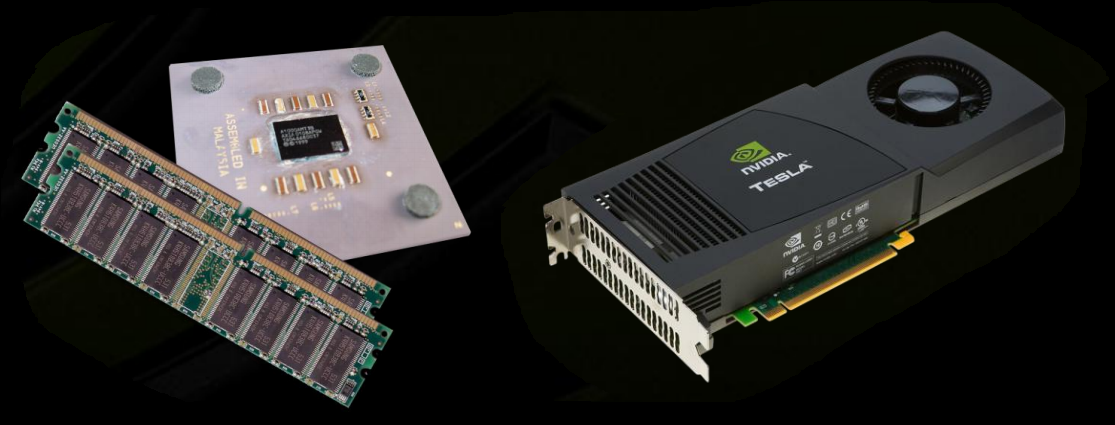
\includegraphics[scale=0.4]{CPU-GPU}

\end{frame}

%------------------------------------------------------------------------------%

\begin{frame}{And the rest?}
\pause

\begin{center}
Don't worry we'll get to that...
\end{center}

\end{frame}

%------------------------------------------------------------------------------%


\begin{frame}
\frametitle{Outline}
\tableofcontents[hideallsubsections,pausesections]
\end{frame}


%##############################################################################%

\section{Background}

\begin{frame}
\tableofcontents[currentsection, hideothersubsections]
\end{frame}

%------------------------------------------------------------------------------%

\subsection{Why?}

\begin{frame}{Why?}

\begin{itemize}[<+->]
\item Special effects are popular in games and movies. 
\item There's always demand for better performance.
\item GPUs are widely available and fairly cheap.
\item \color{green} It's FUN!
\end{itemize}

\end{frame}

%------------------------------------------------------------------------------%

\subsection{Existing Work}

\begin{frame}[t]{Fluids on GPU}

\pause

Interactive SPH Simulation and Rendering on the GPU.
 
\textit{Prashant Goswami}(University of Zurich), 2010.

\vspace{12pt}
\pause

\begin{columns}
\column{.5\textwidth}
\begin{center} 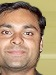
\includegraphics[height=1cm]{Goswami} \end{center}
\pause

\begin{itemize}
\color{white}
\item GPU Based \pause
\item Interactive Framerates \pause
\item Realistic Rendering \pause
\item \alert{No Rigid Bodies!} \pause
\end{itemize}

\column{.5\textwidth}
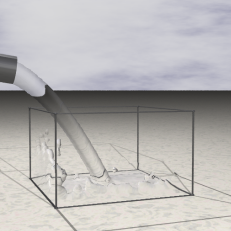
\includegraphics[scale=0.8]{Goswami-Hose}

\end{columns}

\end{frame}

%------------------------------------------------------------------------------%

\begin{frame}[t]{Fluids with Rigid Bodies}

\pause

Versatile Rigid-Fluid Coupling for Incompressible SPH.

\textit{Nadir Akinci}(University of Freiburg), 2012.

\vspace{12pt}
\pause

\begin{columns}
\column{.5\textwidth}
\begin{center} 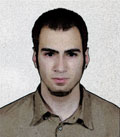
\includegraphics[height=1cm]{Akinci} \end{center}
\pause

\begin{itemize}
\item \color{green} Rigid Bodies \pause
\item \alert{Not GPU!} \pause
\item \alert{Not Realtime!} \pause
\end{itemize}


\column{.5\textwidth}
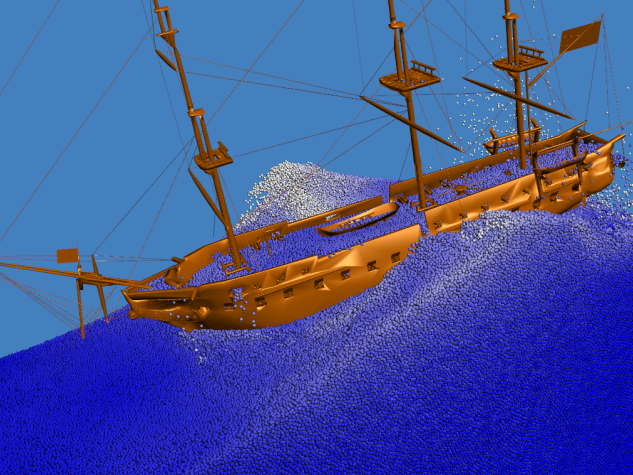
\includegraphics[scale=0.4]{Akinci-Boat}

\pause
\tiny{Wheeeeeeeeeee!!!}

\end{columns}

\end{frame}

%------------------------------------------------------------------------------%

\begin{frame}[plain]{}

\begin{center}
\color{white}
\huge{Time for Another Video...} \vspace{16pt} \pause

\small{YAY!}
\end{center}

\end{frame}


%------------------------------------------------------------------------------%

\subsection{My Plan}

\begin{frame}{So... now what?}

\begin{center}
We have \pause GPU with no rigids \pause and Non-GPU with rigids... \pause

\vspace{16pt}

\huge{\textbf{Combine Them!}}

%\vspace{16pt}
%\pause
%\tiny{kinda...}

\end{center}

\end{frame}

%------------------------------------------------------------------------------%

\begin{frame}[t]{Fluids v.3}

\pause

A Large Scale, Open Source Fluid Simulator Using the Smooth Particle Hydrodynamics Method.

\textit{Rama C. Hoetzlein}, 2012.

%\vspace{16pt}

\pause

\begin{columns}
\column{.5\textwidth}
\begin{center}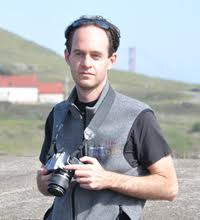
\includegraphics[height=1cm]{Hoetzlein}\end{center} \pause
\column{.5\textwidth}
\color{white} Let's See it First \pause
\end{columns}

\vspace{8pt}

\begin{itemize}
\item GPU Based \pause \checkmark \pause
\item Realtime \pause \checkmark \pause
\item \color{green} Open Source \pause \checkmark \pause
\item \color{orange} No Rigid Bodies \pause (yet...)
\end{itemize}

\pause

\color{white}
\small{I plan to incorporate the method described by Akinci to implement rigid body interaction with fluids \emph{on the GPU.}}


\end{frame}


%------------------------------------------------------------------------------%

\begin{frame}[plain]{}

\begin{center}
But How Does it \emph{Actually} Work?
\end{center}

\end{frame}

%##############################################################################%

\section{Theory}

\begin{frame}
\tableofcontents[currentsection, hideothersubsections]
\end{frame}

%------------------------------------------------------------------------------%

\subsection{SPH Basics}

\begin{frame}{Smoothed Particle Hydrodynamics}
\[
\rho_i=\sum_j m_j W(r_i-r_j,h)
\]
\pause

\begin{center}
\alert{Eeeeeeek!}
\end{center}

\end{frame}


\begin{frame}[t]{Smoothed Particle Hydrodynamics}
\[
\rho_i=\sum_j m_j W(r_i-r_j,h)
\]
\begin{block}{Let's break it down:} 
\pause

\begin{description}[<+->]
\item[$\rho_i$] density of particle \textit{i}  
\item[$m_j$] mass of particle \textit{j}
\item[$W$] \textbf{smoothing kernel}
\item[$r_i-r_j$] distance between particles \textit{i} and \textit{j}
\item[$h$] smoothing cutoff radius
\end{description}

\end{block}

\end{frame}

%------------------------------------------------------------------------------%

\subsection{Smoothing Kernel}

\begin{frame}[t]{Smoothed Particle Hydrodynamics}

\begin{block}{The Smoothing Kernel:}

Must satisfy the following properties:

\vspace{16pt}
\pause

\begin{description}[align=right,labelindent=!]
\item[$\int_\Omega W(r,h)dr=1$] Normalized \pause
\item[$W(r,h)\geq 0$] Positive \pause
\item[$W(r,h)=W(-r,h)$] Symmetric \pause
\end{description}

\vspace{16pt}
\pause
($r$ is inter-particle distance and $h$ is cutoff radius)

\end{block}

\end{frame}

%------------------------------------------------------------------------------%

\begin{frame}[t]{Smoothed Particle Hydrodynamics}

\begin{block}{The Smoothing Kernel:}
Just think of it as a Gaussian curve...

%\vspace{10pt}
\pause

\begin{center}
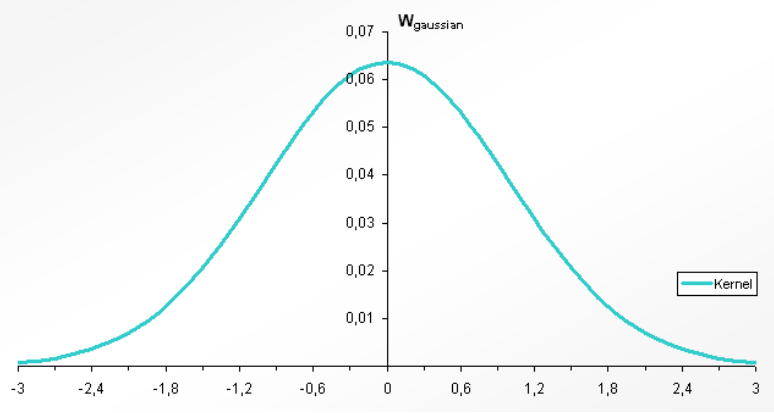
\includegraphics[scale=0.25]{GaussianKernel}

\color{white}
\tiny{Diagram from Kelager[2006]*}
\end{center}

%\vspace{10pt}
\pause

The main point is further particles have less influence... \pause 

and no influence outside the cutoff radius. \pause

\small{\alert{The cutoff radius $h$ is very important!}}


\end{block}

\end{frame}

%------------------------------------------------------------------------------%

\begin{frame}[t]{Smoothed Particle Hydrodynamics}

\begin{block}{The Smoothing Kernel:}

\begin{center}
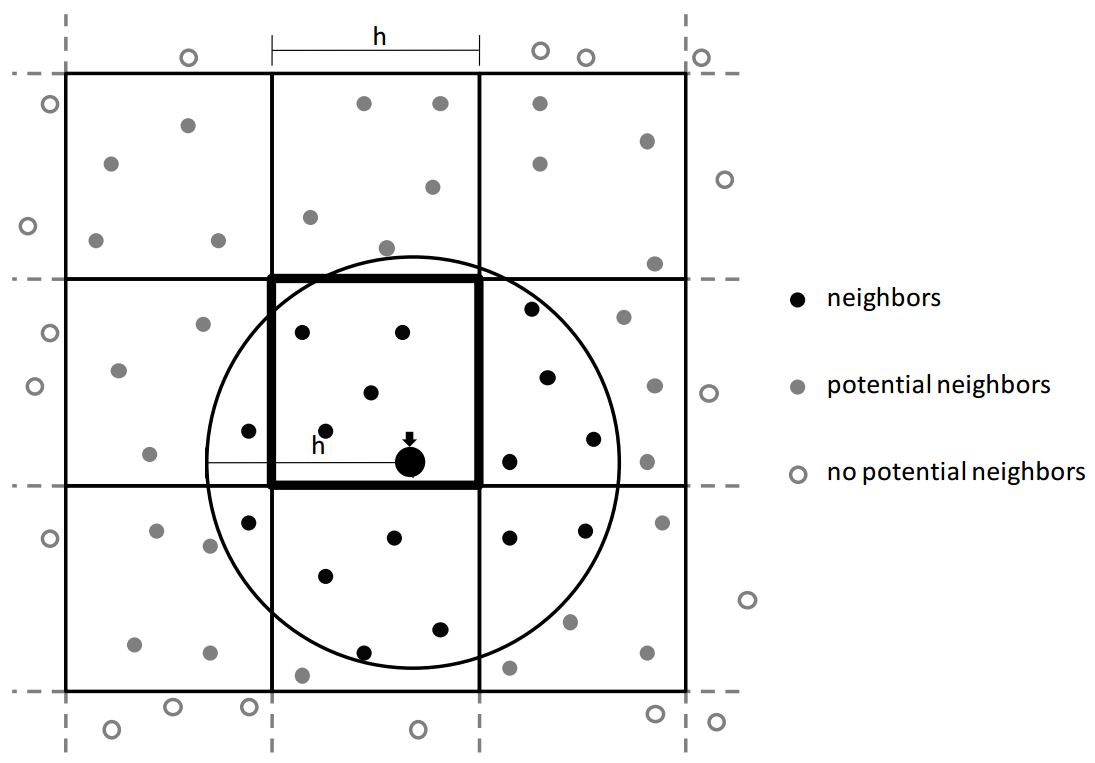
\includegraphics[scale=0.25]{Neighbours}

\color{white}
\tiny{Diagram from: Realtime particle-based fluid simulation, \textit{Stefan Auer}}
\end{center}

\small{\alert{The cutoff radius $h$ is very important!}}

\tiny{\color{white} (we will come back to it in the performance section)}

\end{block}

\end{frame}


%------------------------------------------------------------------------------%

\subsection{Simulation Algorithm}

\begin{frame}[t]{Smoothed Particle Hydrodynamics}

\begin{columns}
\column{.5\textwidth}
\begin{block}{The Algorithm:}
\begin{itemize}

\item To calculate the density of each particle we sum the masses of it's neighbours \pause (weighted by the smoothing kernel $W$). \pause
\item More particles nearby means more density \pause (duh!)

\end{itemize}
\end{block}
\pause

\color{white}
\tiny{* Diagram from: Lagrangian Fluid Dynamics 
Using Smoothed Particle Hydrodynamics, \textit{Micky Kelager} (2006) }

\column{.5\textwidth}


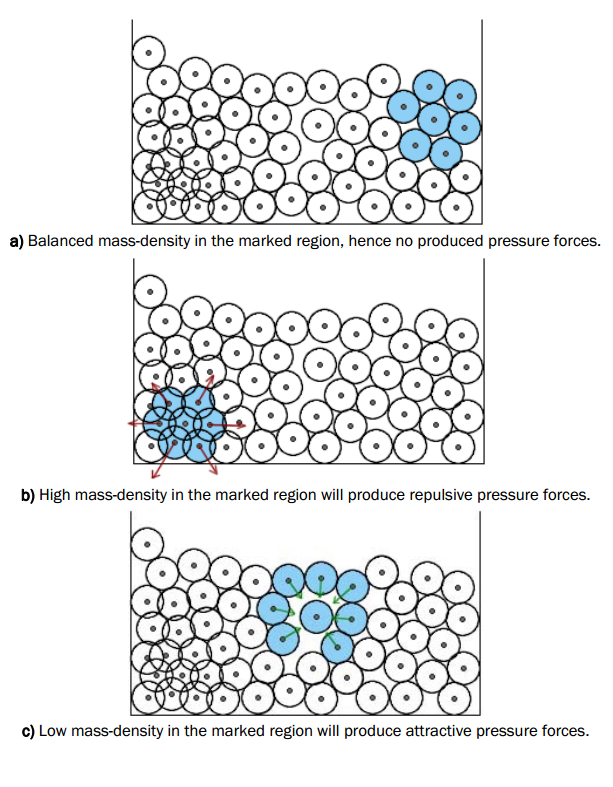
\includegraphics[scale=0.40]{SPH-Theory}

\end{columns}

\end{frame}



%------------------------------------------------------------------------------%

\begin{frame}[t]{Smoothed Particle Hydrodynamics}


\begin{block}{The Algorithm:}

\begin{itemize}
\item Once we have the \emph{density} ($\rho$) surrounding a particle we can calculate the \emph{pressure} ($p$) exerted on it.\pause
\item Using the pressure we can work out the \emph{force} ($f$).\pause
\item From the force we calculate it's \emph{motion}. \pause
\end{itemize}

\begin{center}
\color{white}
\small{Do this for every particle...} \pause \small{every frame...} \pause

\small{And you have a simulation!}
\end{center}

\end{block}

\end{frame}

%------------------------------------------------------------------------------%

\begin{frame}[plain]
\begin{center}
	\huge{\alert{BUT!}} \pause
\end{center}

This gets more expensive the more particles you have... \pause

\begin{center}
\color{white}
And we want \textbf{MILLIONS} of particles! \pause
\end{center}


\small{We'll deal with that in the final section on perfomance. \pause

 For now though...}

\end{frame}

%------------------------------------------------------------------------------%

\subsection{Rigid Body Interaction}

\begin{frame}{What About Those Rigid Bodies?}
\pause

\begin{columns}
\column{.5\textwidth}

\begin{block}{Remember this image:}
\begin{center}
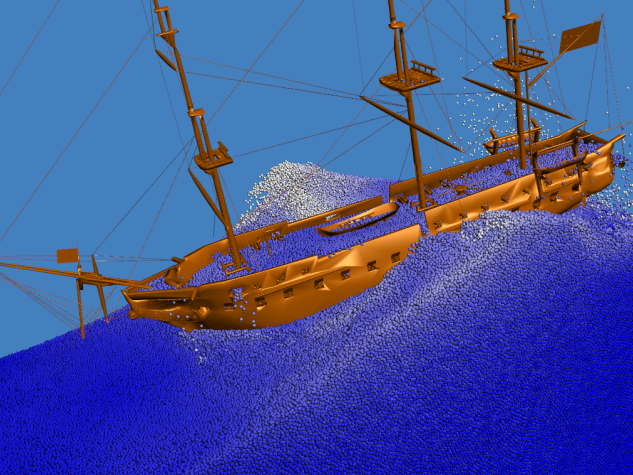
\includegraphics[scale=0.35]{Akinci-Boat}
\end{center}
\end{block}

\pause
\column{.5\textwidth}

\begin{block}{Let's take a closer look:}
\begin{center}
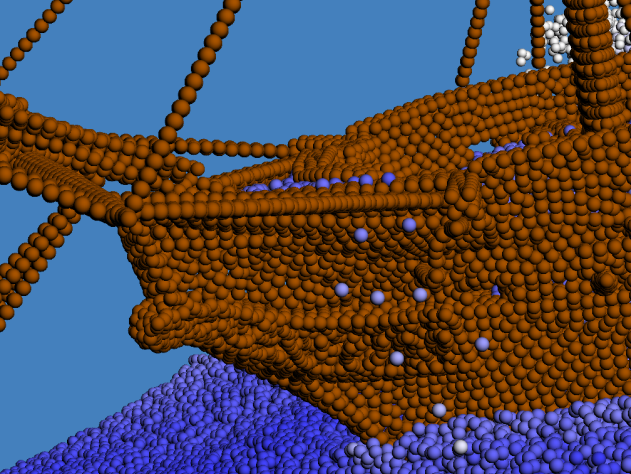
\includegraphics[scale=0.35]{Akinci-Boat-Closeup}
\end{center}
\end{block}

\end{columns}

\pause

See how the boat is made up of particles? \pause

\color{white}
Those are fluid particles... \pause attached to a rigid body!
\end{frame}

%------------------------------------------------------------------------------%

\begin{frame}[t]{The Boat is Made of Fluid Particles... So?}
\pause
Oh yea of little faith :P

\begin{itemize}[<+->]
\item We can use the same algorithm described earlier to calculate the force applied to the boat.
\item We sum the forces from the surrounding fluid particles and apply it to the rigid body.
\item In between simulation steps: rather than letting the attached particles flow, we move the rigid body and update there relative positions.
\item The body is run in Bullet Physics.
\item \color{green} That's it!
\end{itemize}

\end{frame}

%------------------------------------------------------------------------------%

\begin{frame}{Really?}
\pause
No, not really... \pause
We haven't mentioned viscosity! \pause
 
But the principle is similar: \pause

\begin{enumerate}
\item For each particle
\item Accumulate force contributions from neighbours
\item Weight with a smoothing kernel
\item Update
\end{enumerate}

\color{white}
See bonus material at the end for more detail.

\end{frame}

%##############################################################################%

\section{Performance}

\begin{frame}
\tableofcontents[currentsection, hideothersubsections]
\end{frame}

\subsection{Parallelization!}

\begin{frame}{CPU vs GPU}
\pause

A CPU has 4 to 8 powerful cores... \pause A GPU has \emph{hundreds} of simpler ones. \pause

\begin{center}
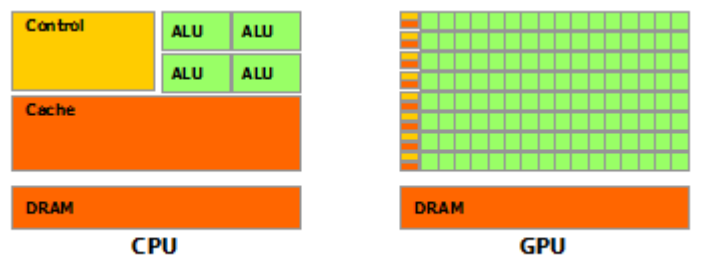
\includegraphics[scale=0.6]{CPU-GPU-Arch}
\end{center}

\color{white}
Remember how we need to process \emph{millions} of particles...

\end{frame}

%------------------------------------------------------------------------------%

\begin{frame}{CPU vs GPU}

\color{white}
Remember we need to process \emph{millions} of particles...

\begin{itemize}[<+->]
\item A CPU has to go through them one by one.
\item \color{green} But a GPU can split up the work!
\item Only because \emph{the same thing} is done to each.
\item \color{orange} (It doesn't work this way for all types of problem!)  
\end{itemize}

\end{frame}

%------------------------------------------------------------------------------%

\begin{frame}[plain]{}

\begin{center}
Parallel is great... \pause

But to get millions of particles... \pause \emph{in realtime}

\vspace{16pt}

\color{white}
\huge{We still have to be \textbf{clever!}}

\end{center}

\end{frame}


%------------------------------------------------------------------------------%

\subsection{Neighbour Search}

\begin{frame}{Let's go back to that cutoff radius...}
\pause 

I did say it was important\pause, so here it is again:

\begin{center}
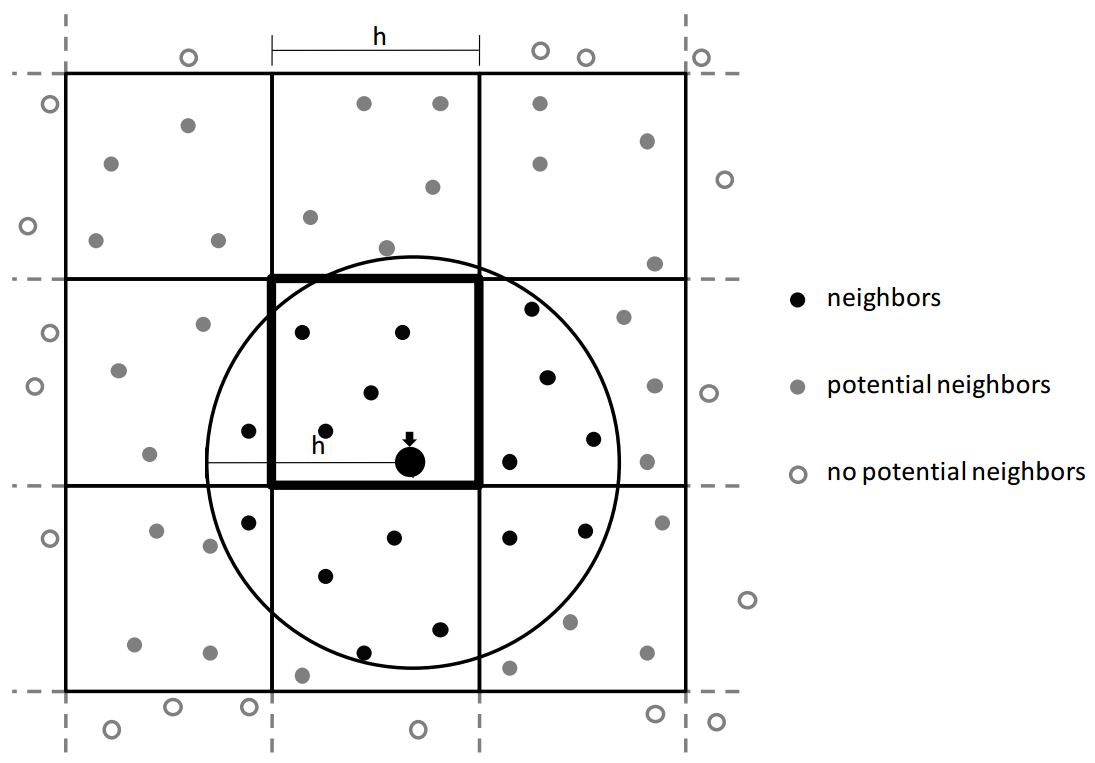
\includegraphics[scale=0.25]{Neighbours}
\end{center}

\pause

We only want to get force from neighbouring particles. \pause 

\color{white}
How do we do that?

\end{frame}

%------------------------------------------------------------------------------%

\begin{frame}[t]{Neighbour Search}
\pause 

\color{white}
Most expensive part of the simulation!

\begin{columns}[t]
\column{.5\textwidth}

\begin{block}{Dumb Way:}

\begin{itemize}[<+->]
\item For each particle.
\item Test every other particle.
\item Ignore if too far away.
\item $O(n^2)$
\end{itemize}

\end{block}

\pause
\column{.5\textwidth}

\begin{block}{Clever Way:}

\begin{itemize}[<+->]
\item Z-Indexing 
\item Groups potential neighbours each timestep.
\item Much fewer tests.
\item \color{green} Also parallelizable!
\end{itemize}

\end{block}

\end{columns}

\pause
\tiny{\color{white} (for more details see [Goswami2010] from earlier) }

\end{frame}

%------------------------------------------------------------------------------%

\subsection{Timestep Size}

\begin{frame}[t]{Timestep Size}
\pause 

\color{white} Biggest performance tradeoff!

\begin{columns}[t]

\pause
\column{.5\textwidth}

\begin{block}{Smaller:}

\begin{itemize}[<+->]
\item More Stable
\item \color{orange} Slower
\end{itemize}

\end{block}

\pause
\column{.5\textwidth}

\begin{block}{Larger:}

\begin{itemize}[<+->]
\item \color{green} Much Faster
\item \color{red} Crazy Artifacts
\end{itemize}

\end{block}

\end{columns}

What can we do?

\end{frame}

%------------------------------------------------------------------------------%

\begin{frame}[t]{PCISPH}
\pause 

\color{white}
Predictive-Corrective \pause Incompressible \pause SPH.

\begin{block}{How does it work?}
Water is uniformly dense so no fluctuations expected. \pause

But with bigger timesteps they are more likely. \pause

So in each step:
\begin{enumerate}[<+->]
\item Predict particle densities before applying velocity.
\item If artifacts occur, correct using a solver.
\item Apply velocity updates.
\end{enumerate}

\end{block}

\tiny{For more details see Predictive-Corrective Incompressible SPH, \textit{Barbara Solenthaler}, 2009}

\end{frame}

%------------------------------------------------------------------------------%

\begin{frame}[t]{Summary}
\pause 

\begin{itemize}[<+->]
\item Incorporate rigid bodies into Hoetzlein's Fluids v.3
\item This will be based on the method from Akinci, 2012
\item Speed it up using GPU parallelization
\item Speed up more with fast neighbour-search and PCISPH 
\end{itemize}

\begin{center}
\color{green} And that's all!
\end{center}

\end{frame}















%------------------------------------------------------------------------------%






\end{document}